\documentclass[tikz,border=10pt]{standalone}
\usetikzlibrary{positioning}
\begin{document}
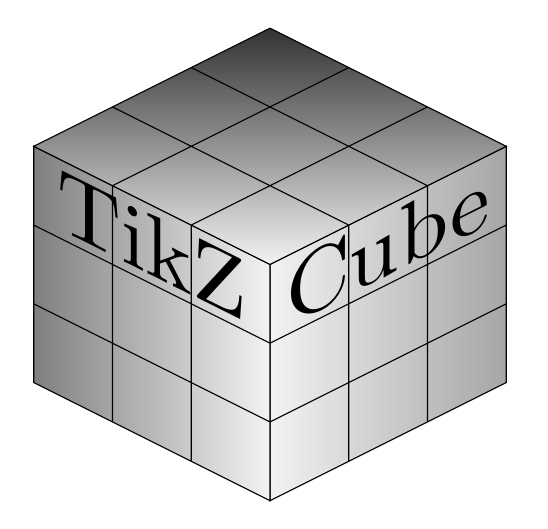
\begin{tikzpicture}
  \draw[yslant=0.5,
    left color=gray!10, right color=gray!70]
    (3,-3) rectangle +(3,3)
    (3,-3)   grid    +(3,3);
  \draw[yslant=-0.5,
    left color=black!50, right color=gray!10]
    (0,0) rectangle +(3,3)
    (0,0) grid +(3,3);
  \draw[yslant=0.5,xslant=-1,
    bottom color=gray!10, top color=black!80]
    (3,0) rectangle +(3,3)
    (3,0) grid +(3,3);
  \node[yslant=-0.5, scale=3.2]
    at (1.5,1.75) {TikZ};
  \node[yslant= 0.5, scale=3.2]
    at (4.5,1.75) {Cube};
\end{tikzpicture}
\end{document}
